\documentclass{article}
\usepackage{graphicx}
\title{Engineering Design Process}
\author{Dr. Keith Evan Schubert\\ Baylor University}
\begin{document}
\maketitle

%\chapter{Engineering Research}



\section{Formal Techniques}

Probably the most famous techniques are the Waterfall method and the `V' method.  Both are very similar.  The Waterfall technique is based on the idea that one phase flows to the next.  It develops a systems life cycle that we will discuss below.  The `V' method is similar, but folds the testing in the second half of the life cycle up to pair it with the spec development of the first half.  Thus the detailed designs at the end pair with unit tests of the parts that were designed, and the customer requirements and the very beginning pair with acceptance tests.  Full formal techniques are only done on major projects such as military projects that require such a high level of oversight and no easy breakdown is possible, but the concepts are super helpful to understand.  Good references (available online) are the Defense Acquisition Guidebook and the Defense System Software Development book.  The overall process is :%illustrated in Figure~\ref{

%\begin{figure}
%\begin{center}
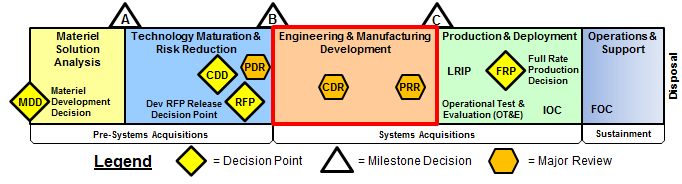
\includegraphics[width=0.9\textwidth]{graphics/EMD-Acquisition-System.png}
%\caption{Engineering and Manufacturing Development (EMD) phases.}\label{fig:EMD}
%\end{center}
%\end{figure}

Gantt Charts:

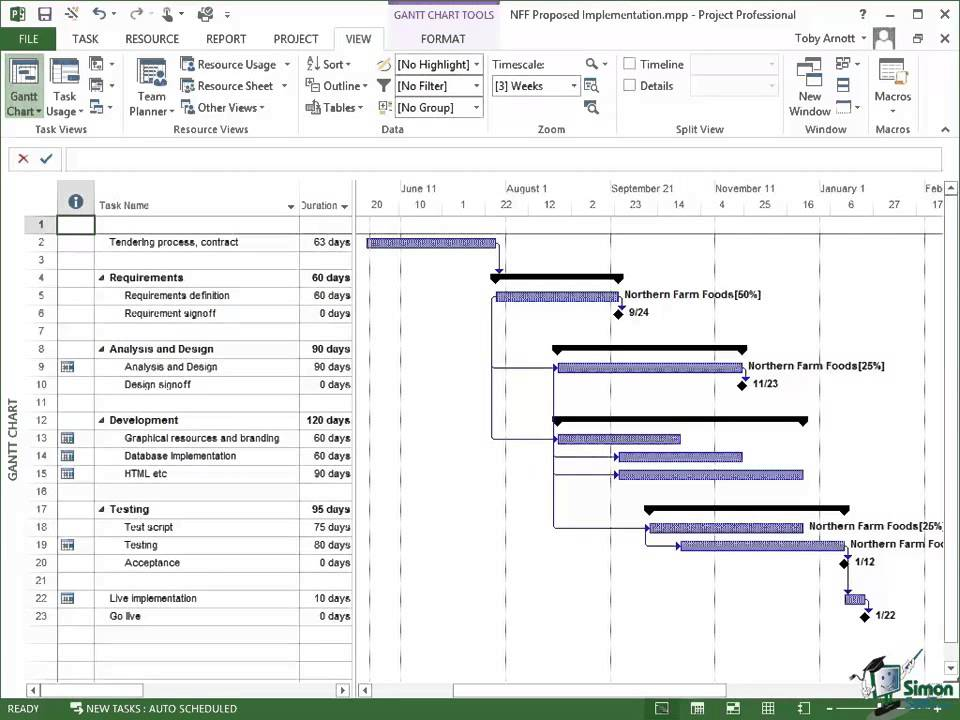
\includegraphics[width=0.9\textwidth]{graphics/gantt.jpg}

\section{Agile Techniques - SCRUM}

Agile methods are designed to switch from large, formal processes that are run top-down to small, flexible ones that are run bottom-up.  While hierarchical (top-down) methods have historic dominance, Agile techniques dominate now, and their flexibility and creativity are likely to keep them on top for a while.  They are far from free of criticism, and though I personally like them, I am more of a hybrid techniques person.

%\subsection{SCRUM}


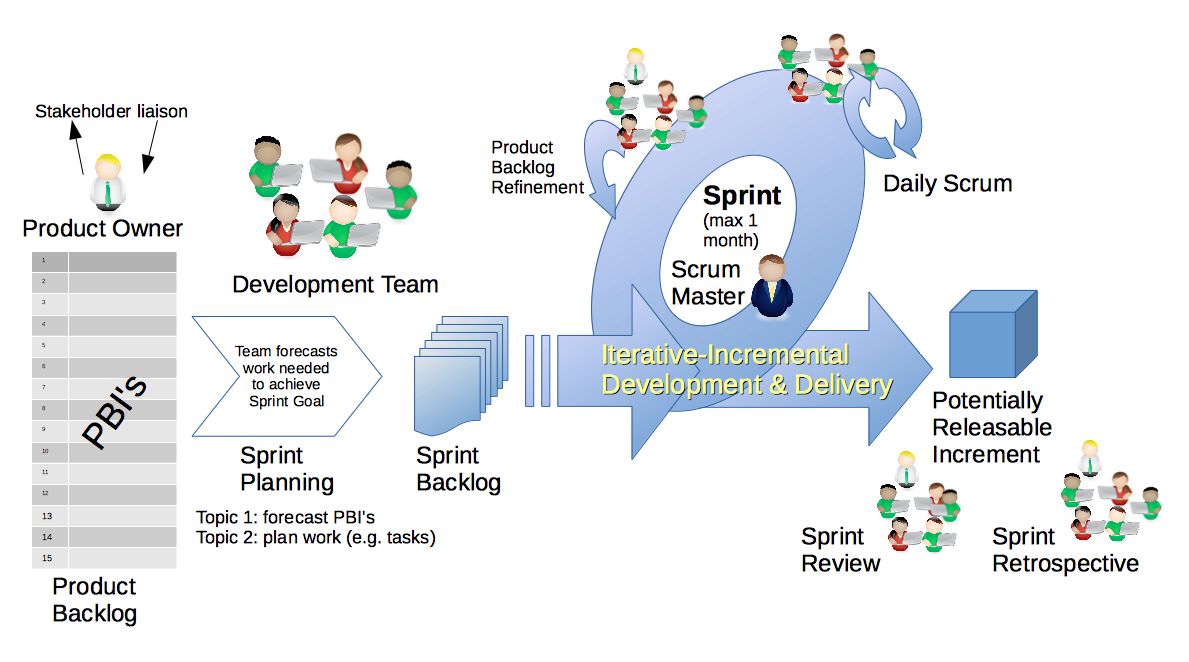
\includegraphics[width=0.9\textwidth]{graphics/Scrum_Framework.png}

%Sprint - The current development and delivery

Daily scrum - a daily meeting of the team to quickly establish goals for the day.  Quick is important- the meeting for the team is ideally around 15 min.  To enforce this the meeting is standing only - no chairs or places to lean.  Meetings are often held in a place that would be awkward to keep going too long, like the isle of the team work area.  The goal is not to tell your life story but establish daily goals and deliverables.  If help is needed that can get assigned in the daily goals.  You answer 3 questions in about 1-2 min:
\begin{enumerate}
\item What did you do yesterday?
\item What are you doing today?
\item What problem (impediment, risk) is blocking you?
\end{enumerate}

Scrum master - the lead of the project in some sense, but the goal of the scrum master is to remove impediments of the team, and buffer from distractions. The position is sometimes described as a facilitator or a servant-leader, and it is this second description that really resonates with me, as this is what Jesus did, and what He calls each of us to do.  Micro-managing doesn't work.

Burndown Charts:


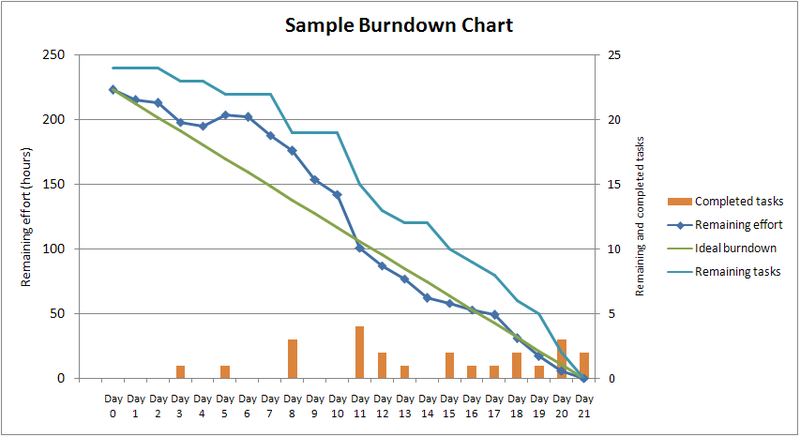
\includegraphics[width=0.9\textwidth]{graphics/BurndownChart.png}

Scrum task board:


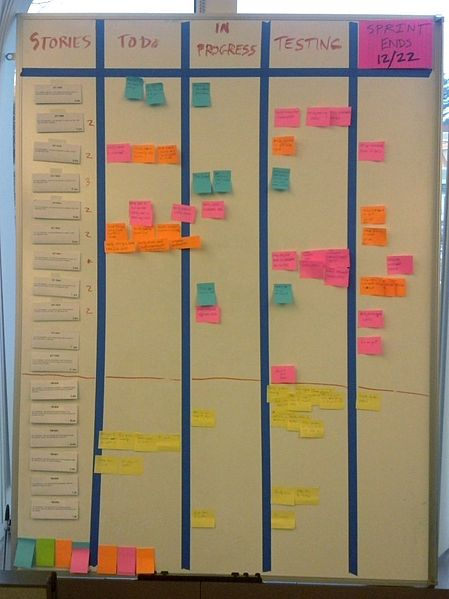
\includegraphics[width=0.9\textwidth]{graphics/Scrum_task_board.jpg}




\end{document} 